\documentclass[pdf, handout]{beamer}
\mode<presentation>{\usetheme{Warsaw}}
%% preamble
 \setbeamertemplate{headline}{}
\setbeamertemplate{section page}[mine]
% \setbeamertemplate{footline}[]
\title{Risk Measurement and Management \\
using the greeks}
\subtitle{Quantitative Finance}
\author{Tilburg University}
\institute{Ramon van den Akker}
\date{}
%%
\usepackage{array}
\usepackage{multirow}

%\newcommand\MyBox[2]{
%  \fbox{\lower0.75cm
%    \vbox to 1.7cm{\vfil
%      \hbox to 1.7cm{\hfil\parbox{1.4cm}{#1\\#2}\hfil}
%      \vfil}%
%  }%
%}



%%%%%%%%%%%%%%%%%%%%%%%%%%%%%%%%%%%%%%%%%%%%%%%%%%%%%%%%%%%%%%%%%%%%%%%%%%%%%%%%%%%%%%%%%%%%%%%%%%%%%%%%%%%%%%%%%%%%%%%%
%%%%%%%%%%%%%%%%%%%%%%%%%%%%%%%%%%%%%%%%%%%%%%%%%%%%%%%%%%%%%%%%%%%%%%%%%%%%%%%%%%%%%%%%%%%%%%%%%%%%%%%%%%%%%%%%%%%%%%%%
%%%%%%%%%%%%%%%%%%%%%%%%%%%%%%%%%%%%%%%%%%%%%%%%%%%%%%%%%%%%%%%%%%%%%%%%%%%%%%%%%%%%%%%%%%%%%%%%%%%%%%%%%%%%%%%%%%%%%%%%
%\usepackage{diagrams}
\usepackage{amsmath}
%\usepackage{graphics}
\usepackage{multicol}
\usepackage{subfigure}
\usepackage{graphicx}
\usepackage{pstricks}
\input{commands.txt}
%\renewcommand{\E}{\operatorname{E}}
\newcommand{\Var}{\operatorname{Var}}
\renewcommand{\epsi}{\varepsilon}
\newcommand{\argmin}{\mathop{\mathrm{arg\,min}}}
\newcommand{\rank}{\operatorname{rank}}
\renewcommand{\kansp}{\mathbb{P}}
\renewcommand{\calF}{\mathcal{F}}
\newcommand{\e}{\operatorname{e}}
\newcommand{\Bin}{\operatorname{Bin}}
\newcommand{\kbin}{\operatorname{b}}
\newcommand{\lin}{\operatorname{lin}}
\newcommand{\kansq}{\mathbb{Q}}
%\newarrow{hulp}{<}{filler}{middle}{filler}{head}
\DeclareMathOperator*\ster{*} \DeclareMathOperator*\argmax{argmax}
\usepackage{color}
%%%%%%%%%%%%%%%%%%%%%%%%%%%%%%%%%%%%%%%%%%%%%%%%%%%%%%%%%%%%%%%%%%%%%%%%%%%%%%%%%%%%%%%%%%%%%%%%%%%%%%%%%%%%%%%%%%%%%%%%
%%%%%%%%%%%%%%%%%%%%%%%%%%%%%%%%%%%%%%%%%%%%%%%%%%%%%%%%%%%%%%%%%%%%%%%%%%%%%%%%%%%%%%%%%%%%%%%%%%%%%%%%%%%%%%%%%%%%%%%%
%%%%%%%%%%%%%%%%%%%%%%%%%%%%%%%%%%%%%%%%%%%%%%%%%%%%%%%%%%%%%%%%%%%%%%%%%%%%%%%%%%%%%%%%%%%%%%%%%%%%%%%%%%%%%%%
%
%
%
%

%
%\begin{frame}{}
%Fundamental assumption: \\
%NO FREE LUNCH WITHOUT RISK\bigsqcup
%\end{frame}

\AtBeginSection{\frame{\sectionpage}}
%\AtBeginSubsection{\frame{\subsectionpage}}
\newtranslation[to=greek]{Section}{En'othta}
\newtranslation[to=greek]{Subsection}{Upoen'othta}

\defbeamertemplate{section page}{mine}[1][]{%
  \begin{centering}
    {\usebeamerfont{section name}\usebeamercolor[fg]{section name}#1}
    \vskip1em\par
    \begin{beamercolorbox}[sep=12pt,center]{part title}
      \usebeamerfont{section title}\insertsection\par
    \end{beamercolorbox}
  \end{centering}
}

\defbeamertemplate{subsection page}{mine}[1][]{%
  \begin{centering}
    {\usebeamerfont{subsection name}\usebeamercolor[fg]{subsection name}#1}
    \vskip1em\par
    \begin{beamercolorbox}[sep=8pt,center,#1]{part title}
      \usebeamerfont{subsection title}\insertsubsection\par
    \end{beamercolorbox}
  \end{centering}
}

%%
\begin{document}
% title frame
\begin{frame}
\titlepage
\end{frame}
%


%%%%%%%%%
\section{Introduction}
%
%%
\begin{frame}{Motivation: solving valuation problem is not enough}
\begin{itemize}
\item suppose we work at bank ABC which acts
as market-maker 
\item customer S contacts us to buy 10,000 European call options
on Air France-KLM which expire in 3 months from now and have 
5 euro as strike price
\begin{itemize}
\item assume that such European options are not traded on exchanges
\end{itemize}
\item bank ABC steps in, to facilitate the needs of S, and offers to sell (write) the option
\item using their models $10,000\times 0.30 = 3,000$ euro is the no-arbitrage price for the options
\item reasonable commerical price is: $3,000$ euro + fee 
(to be received at $t=0$)
\item we have solved the valuation problem for bank ABC
\end{itemize}
\end{frame}

\begin{frame}{Motivation: solving valuation problem is not enough}
Suppose bank ABC takes no further action. Then at $t=3/12$:
\begin{itemize}
\item if stock price at $t=3/12$ is below 5 euro:
\begin{itemize}
\item there are no additional cashflows [profit=$3,000\times\exp(rT)$] 
\end{itemize}
\item if stock price at $t=3/12$ exceeds 5 euro:
\begin{itemize}
\item bank ABC needs to sell stocks to S for $5$ euro; this leads to loss
of $10,000 \times (S_{3/12} -5) - 3,000\times\exp(rT)$ euro
\item note that potential loss is unbounded (assuming GBM as model for $S$):  for any $K>0$:  $\mathbb{P}(S_{3/12} > K)>0$
\end{itemize}
\item so selling the option yields risk. Bank ABC would like (and is enforced to do so by regulators) to \emph{measure}  the risk
and bank ABC might want to \emph{manage} the risk by hedging part of the risk (because of its own risk appetite or because of regulatory limits)
\item we will discuss risk measurement and hedging using the greeks
\item our discussion is very specific to option portfolios; see MSc in QFAS for wide-range of tools for risk measurement and management
\end{itemize}
\end{frame}

%
%\begin{frame}{Valuation and Hedging example}
%Suppose bank uses 400,000 euro as forward price and proceeds as follows:
%\\ \vspace{.3cm}
%\textbf{No hedge at all} 
%\begin{itemize}
%\item if stock price at $t=3/12$ is below 4 euro:
%\begin{itemize}
%\item profit  $100,00 \times (4 -S_{3/12})$ 
%\end{itemize}
%\item if stock price at $t=3/12$ exceeds 4 euro:
%\begin{itemize}
%\item loss  $100,00 \times (S_{3/12} -4)$
%\item note that potential loss is unbounded (assuming GBM as model for $S$):  for any $K>0$:  $\mathbb{P}(S_{3/12} > K)>0$
%\end{itemize}
%\end{itemize}
%\textbf{Full hedge}
%\begin{itemize} 
%\item using strategy on previous slide we always have
%$400,000 - 385,208$ euro as profit at $t=3/12$ (without any other net cashflows)
%\end{itemize}
%\end{frame}
%

\begin{frame}{Hedging}
\begin{itemize}
\item Cambridge Dictionary describe \textbf{hedging}  as
\begin{quote}
`the activity of reducing the risk of losing money on shares, bonds, etc. that you own'
\end{quote}
\item In finance we have many concepts and techniques to reduce risk. Some examples from the point-of-view of an investor:
\begin{itemize}
\item using \emph{diversification}  in investment portfolio  (e.g. Markowitz portfolio theory)
\item buying specific contracts to eliminate or reduce risk(s)
in your porfolio
(e.g. buy put option in combination with stock)
\end{itemize}
\item This topic takes point-of-view 
of (trading desk of)  financial institution that sells (writes)
(non-traded) European
options 
\begin{itemize}
\item yields incoming cashflow (premia) at inception
\item yields liability at maturity/expiration date
\item liability at maturity yields risk
\item institution might want to hedge (part of) the risk
\end{itemize}
\end{itemize}
\end{frame}





\begin{frame}{Agenda}
These slides discuss hedging of option portfolios from
point-of-view 
of (trading desk) of financial institution 
that sells (writes)
(non-traded) European
options 
\begin{itemize}
\item we will use continuous-time model for financial market, but will acknowledge that we can only trade on discrete time-grid 
\item in this discussion we will focus on using/exploiting closed-form formulas for
option prices and related objects
\end{itemize}
In the next section we first reconsider situation
in which  we assume that we can trade in continuous-time
\end{frame}

\section{Hedging in continuous time}

\begin{frame}{Replicating portfolio}
For the Black-Scholes market we have obtained:
\begin{itemize}
\item if we have option with price process $C_t=F(t, S_t)$,
then  $F$ satisfies
\[
\frac{\delta F}{\delta t}(t,s) + r s \frac{\partial F}{\partial
s}(t,s) + \frac{1}{2}\sigma^2 s^2 \frac{\partial^2 F}{\partial
s^2}(t,s) -r F(t,s)=0\quad \forall s,t
\]
\item there is self-financing portfolio $(\phi_t,\psi_t)_{t\geq 0}$ that replicates payoff option, i.e. $C_T=V_T=\phi_T S_T+ \psi_T B_T$, given by:
\begin{align*}
\phi_t &=\frac{\partial F}{\partial s}(t,S_t) \\
\psi_t &=\frac{F(t, S_t)-\phi(t,S_t) S_t}{B_t}
\end{align*}
\end{itemize}
\end{frame}

\begin{frame}{Perfect hedge}
\begin{itemize}
\item suppose financial institution sells option to customer
\item receives price/premium option at $t=0$
\item needs to pay $C_T\geq 0$ at maturity
\item if institution does not want to have any exposure to risk:
\begin{itemize}
\item setup self-financing trading strategy (from previous sheet) at $t=0$
\item costs $C_0$ at $t=0$
\item the self-financing portfolio replicates payoff $C_T$ at maturity 
$\implies$ no net cashflow at time $T$
\item self-financing $\implies$ no intermediate net cashflows
\item charging price $C_0$ + `additional fee' yields positive cashflow without any risk
(at $t=0$)
\end{itemize}
\end{itemize}
\end{frame}


\begin{frame}{Illustration}
\begin{itemize}
\item Consider Black-Scholes market with $S_0=100$, $r=1\%$, $\mu=5\%$, $\sigma=20\%$ and European option with maturity $T=3$
and payoff $1,000\times \max\{K-S_T,0\}$ with $K=90$ (i.e. 1,000 put options)
\item a realization:
\begin{figure}
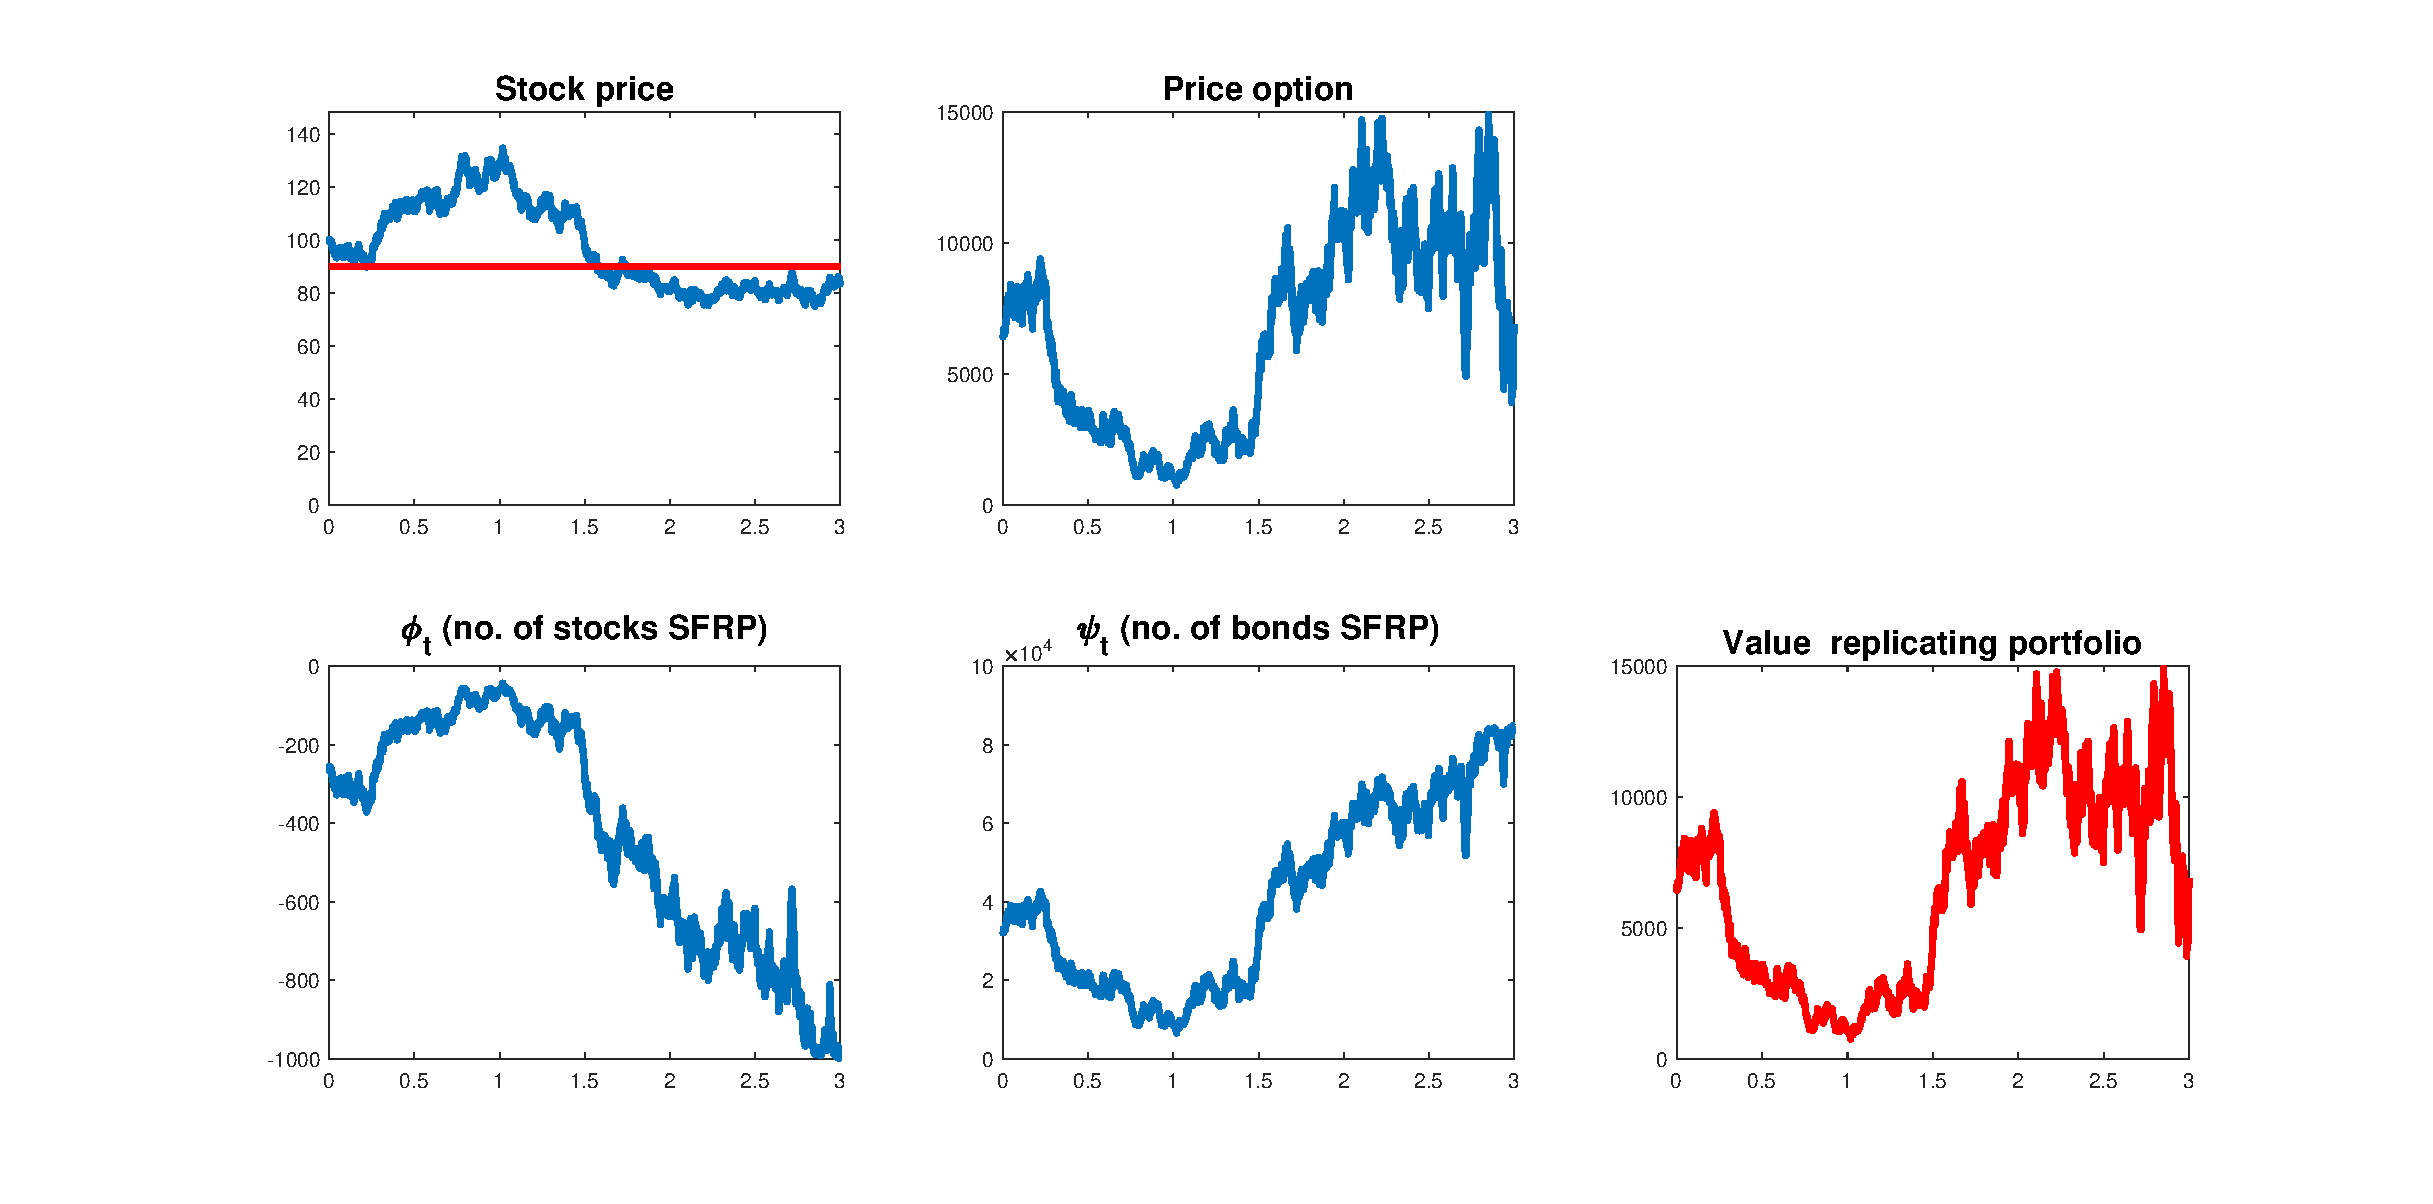
\includegraphics[width=0.85\textwidth]{illu_put.eps}
\end{figure}
\end{itemize}
\end{frame}

\begin{frame}{Illustration - remarks}
\begin{itemize}
\item positions in self-financing porfolio look very wiggly
\item we can show:
\[
\phi_t = - 1,000 \Phi(-d_1)  
\]
with
\[
d_1 =
\frac{
\log(S_t/K)+(r +0.5 \sigma^2)(T-t)}{\sigma\sqrt{T-t}}
\]
\item recall
\[
S_t = S_0 \exp( (\mu-0.5\sigma^2) t + \sigma W_t^{\mathbb{P}})
\]
so we see that $\phi_t$ is non-differentiable function of time
\end{itemize}
\end{frame}

\begin{frame}{Reflection}
The previous results strongly depend on the assumption that we can trade in continuous time...
\\ \vspace{.5cm}
How to proceed if we only trade
on discrete time-grid (e.g. daily)?
\end{frame}

\section{Hedging in discrete time and the greeks}

\begin{frame}{Setup}
\begin{itemize}
\item suppose we have sold (European) option with payoff 
$C_T$ at maturity $T$
\item price $C_t = F(t,S_t)$  at time $t$
\item note that $F$ will also depend on parameters
\begin{itemize}  
\item in case of European put/call and Black-Scholes market:  $F(t,S_t) =F(t,S_t; T, K, r,\sigma)$
\end{itemize}
\item we do not want to/cannot trade in continuous time, only 
on discrete-time grid (e.g. daily)
\item we want to hedge exposure to risk; how to proceed?
\item It\^{o} suggests that change in option price over time interval
$[t, t+\epsilon]$ is given by:
\begin{align*}
C_{t+\epsilon} -C_t  & 
\approx
 F_S(t,S_t)\times \Delta S_{t+\epsilon} 
+ F_t(t,S_t)\times \epsilon \\
&\quad +\frac{1}{2} F_{SS}(t,S_t) \times 
\left(\Delta S_{t+\epsilon}\right)^2
\end{align*}
\end{itemize}
\end{frame}


\begin{frame}{Delta}
\begin{itemize}
\item we have
\begin{align*}
C_{t+\epsilon} - C_t 
&\approx
F_S(t,S_t)\times \Delta S_{t+\epsilon} 
+ F_t(t,S_t)\times \epsilon \\
&\quad +\frac{1}{2} F_{SS}(t,S_t) \times 
\left(\Delta S_{t+\epsilon}\right)^2
\end{align*}
\item for any portfolio with price process $V_t=G(t,S_t)$ we define
\textbf{Delta} by:  
\[
\Delta=\Delta_t =\left. \frac{\partial }{\partial s} G(t,s)\right|_{s=S_t} = G_S(t,S_t)
\]
\item portfolio for which $\Delta$ (at time $t$) is equal to 0 is called \textbf{delta neutral}  (at time $t$)
\item in case of small changes in stock price delta-neutral portfolios have limited (local) risk
\end{itemize}
\end{frame}

\begin{frame}{Delta}
\begin{itemize}
\item for Black-Scholes market the Delta of European call and put option are given by
\[
\Delta_{\text{call}} = \Phi(d_1) \text{  and } 
\Delta_{\text{put}} = -\Phi(-d_1)
 \]
with
\[
d_1= \frac{
\log(S_t/K)+(r +0.5 \sigma^2)(T-t)}{\sigma\sqrt{T-t}}
\]
\item portfolio consisting of $a$ options and $b$ stocks (at time $t$) has Delta:
\[
\Delta_{\text{portfolio}} = a \Delta_{\text{option}}
+ b  
\]
\item to obtain delta-neutral portfolio at time $t$ we 
set $b = - a \Delta_{\text{option}}$
\item activity of obtaining delta-neutral portfolio
is called \textbf{delta hedging}
\end{itemize}
\end{frame}

\begin{frame}{Delta-hedging in continuous-time}
\textbf{Remark}
\begin{itemize}
\item go back to continuous-time framework for the moment
\item note that the $\Delta$ of the option corresponds to the
position, in the stock, in the self-financing replicating portfolio!
\item so in continuous-time we can perform delta-hedging using
a self-financing portfolio
\item only applying this hedge at discrete points-in-time
destroys, in general, the self-financing property! Or: if we want to have 
self-financing portfolio in discrete time we are, in general, not able
to replicate the payoff of the option without error
(as we will see in simulations)!
\end{itemize}
Now back to trading on a discrete time grid.
\end{frame}




\begin{frame}{Delta-hedging with self-financing portfolio}
\begin{itemize}
\item supose we have $a$ options, against price $C_0$
\item take a position in stock and money market to obtain delta-neutral portfolio at $t=0$ such that total portfolio is delta-neutral and has value 0
\item at each point-in-time 
we rebalance the position in $S$ such that the total 
portfolio is delta-neutral: for $t=\eta, 2\eta,\dots,(n-1)\eta$, with $n\eta=T$,
\[
\phi_t=  - a\Delta_{\text{option}, t} 
\]
We want to rebalance positions in $(S,B)$ in a budget-neutral way, i.e.
\[
\psi_t = (\phi_{t-\eta} S_t + \psi_{t-\eta} B_t- \phi_t S_t )/B_t
\]
\item at maturity the total portfolio has payoff
\[
aC_T + \phi_{T-\eta} S_T + \psi_{T-\eta} B_T 
\]
which in general wil differ from 0, i.e. we have replication error
(due to rebalancing in discrete-time instead of continuous time)!
\end{itemize}
\end{frame}

\begin{frame}{Illustration}
\begin{itemize}
\item consider Black-Scholes market with $S_0=100$,
$r=1\%$, $\mu=5\%$, $\sigma=20\%$ and European option with maturity $T=1$
and payoff $1,000\times \max\{K-S_T,0\}$ with $K=90$ (i.e. 1,000 put options)
\item no arbitrage price: 3,297 euro
\item simulation-based approximation to distribution (real world)
of $S_T$ (10,000 replications)
\begin{figure}
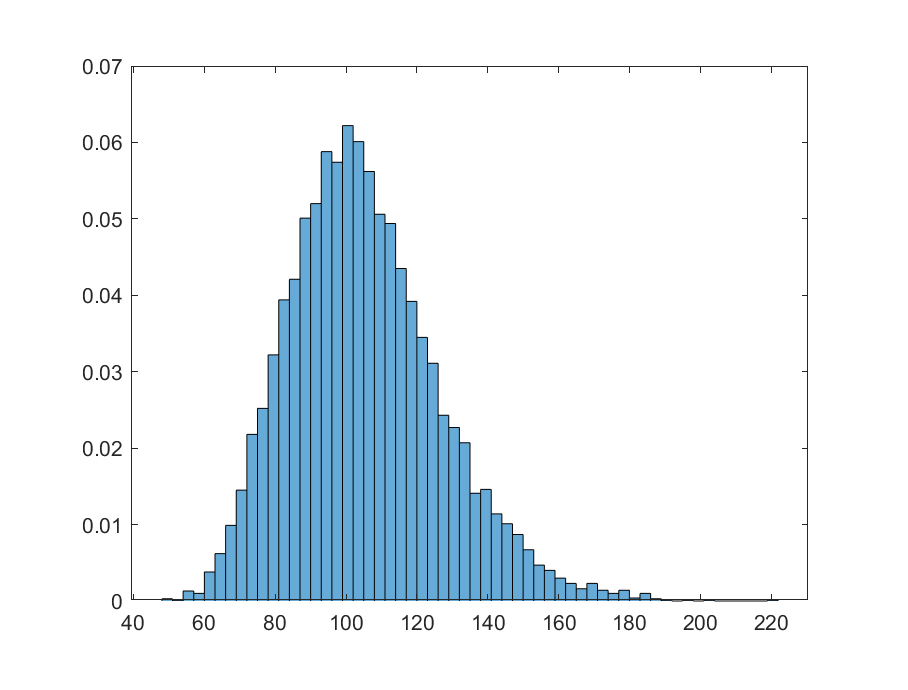
\includegraphics[width=0.6\textwidth]{distr_ST.eps}
\end{figure}
\end{itemize}
\end{frame}

\begin{frame}{Illustration}
\begin{itemize}
\item simulation-based approximation to distribution (real world)
of $C_T$ (10,000 replications)
\begin{figure}
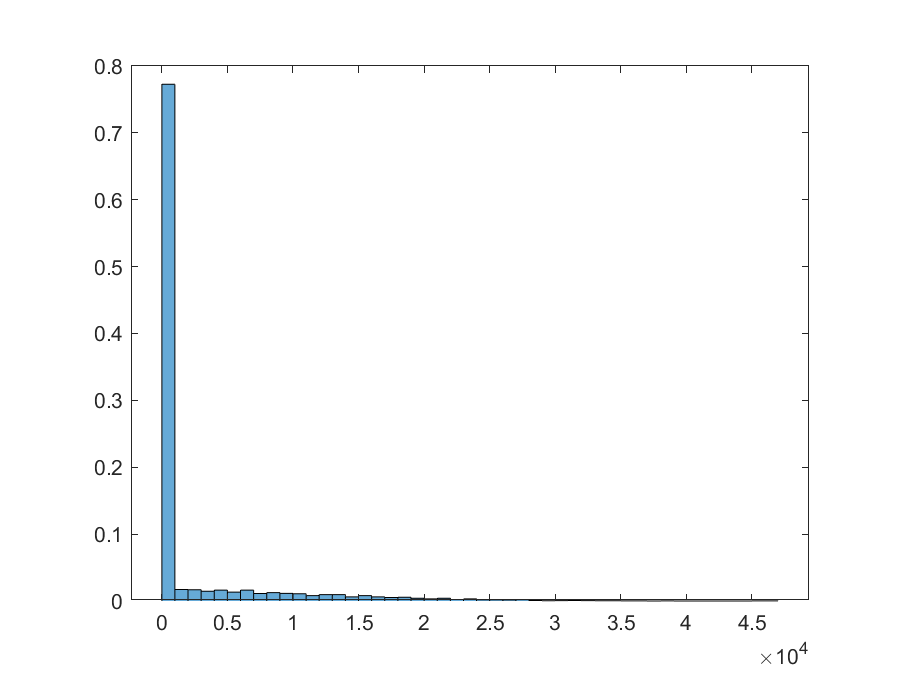
\includegraphics[width=0.65\textwidth]{distr_CT.eps}
\end{figure}
mean: 2,429 euro, $95\%$-quantile: 16,035 euro
\end{itemize}
\end{frame}

\begin{frame}{Illustration}
\begin{itemize}
\item simulation-based approximation to distribution (real world)
of hedge/replication error at maturity $T$ (10,000 replications)
\begin{figure}
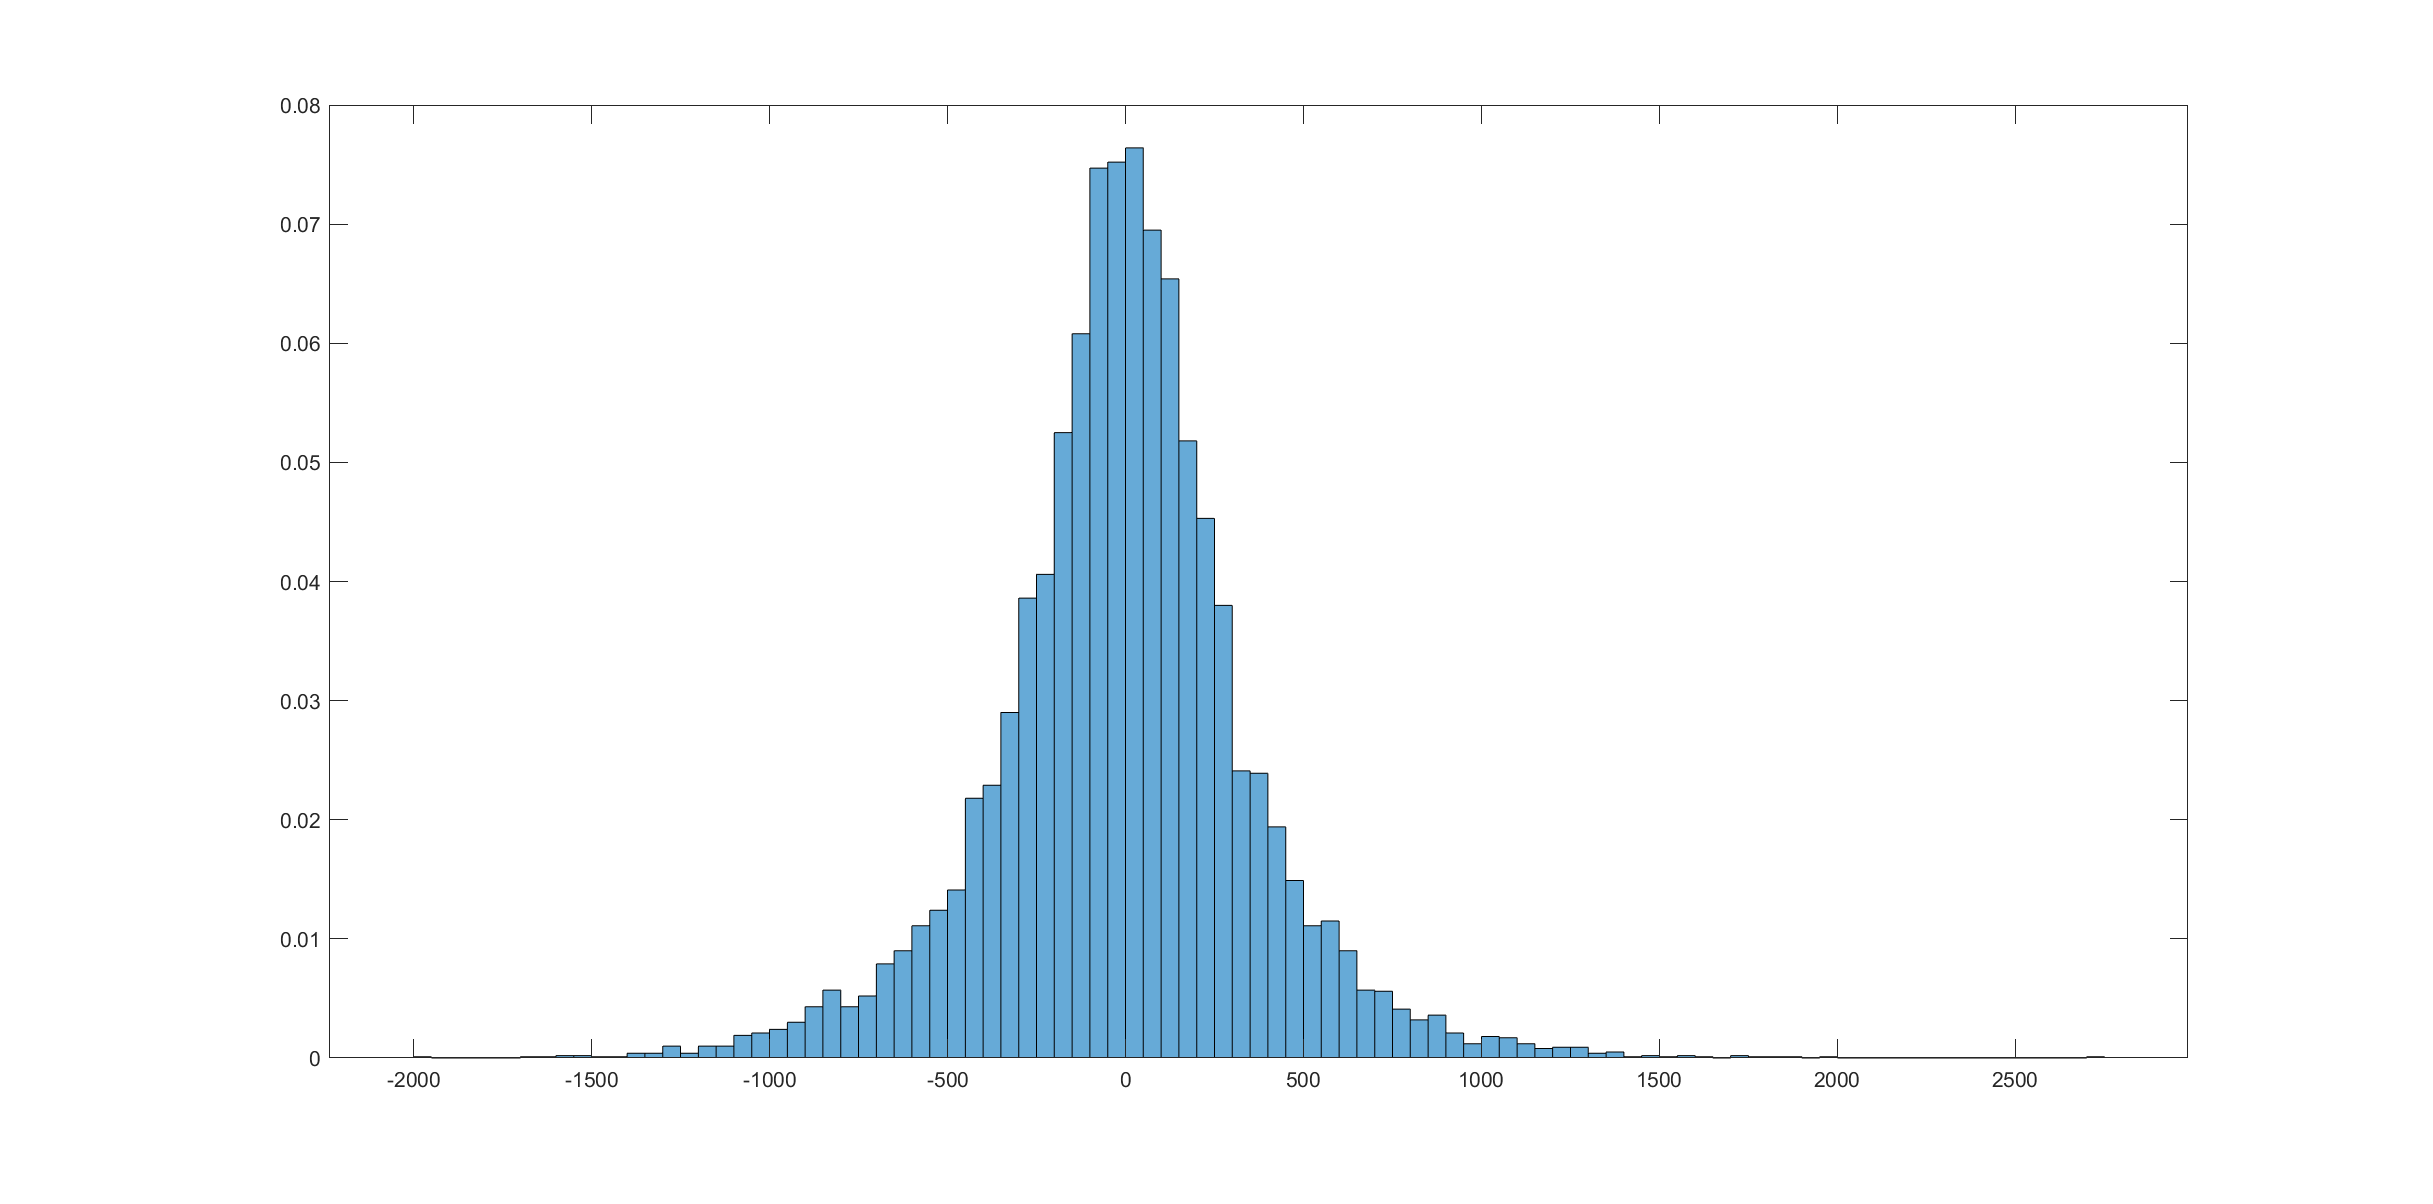
\includegraphics[width=0.95\textwidth]{distr_hedge_error.eps}
\end{figure}
\end{itemize}
So by using the ``self-financing delta-neutral'' hedge we have substantially reduced the risk at maturity $T$ (without cost)
\end{frame}

\begin{frame}{Gamma}
\begin{itemize}
\item Recall that ``delta'' was motivated by
approximation to change in portfolio value
\begin{align*}
V_{t+\eps}-V_t
&\approx
 \frac{\partial V}{\partial S_t}(t,S_t)\times \Delta S_{t+\epsilon} 
+\frac{\partial V}{\partial t}\times \epsilon 
%\\ &\quad 
+\frac{1}{2} \frac{\partial^2 V}{\partial S_t^2} \times 
\left(\Delta S_{t+\epsilon}\right)^2
\end{align*}
\item higher order term might
be relevant as well $\implies$ gamma 
\end{itemize}
For any portfolio with price process $V_t=G(t,S_t)$ we define
\textbf{Gamma} by:  
\[
\Gamma=\Gamma_t =\left. \frac{\partial^2 }{\partial s^2} G(t,s)\right|_{s=S_t} = G_{SS}(t, S_t) =\frac{\partial}{\partial s} \left. \Delta_t
\right|_{s=S_t}
\]
Note that gamma (also) measures direction of $\Delta$. 
Portfolio for which $\Gamma$ (at time $t$) is equal to 0 is called \textbf{gamma neutral}  (at time $t$).
\end{frame}

\begin{frame}{Gamma}
\begin{itemize}
\item 
for Black-Scholes market the gamma of European call and put option are given by
\[
\Gamma_{\text{call}} = 
\Gamma_{\text{put}} = \frac{1}{S_t\sigma\sqrt{T-t}}\phi(d_1)
 \]
with
\[
d_1= \frac{
\log(S_t/K)+(r +0.5 \sigma^2)(T-t)}{\sigma\sqrt{T-t}}
\]
\item portfolio consisting of $a$ options I, $b$ stocks, and $c$ options II (at time $t$) has Gamma:
\[
\Gamma_{\text{portfolio}} = a \Gamma_{\text{option I }}
+c \Gamma_{\text{option II}}
\]
$\implies$ if we sell non-traded option, we can obtain \textbf{gamma-neutral} portfolio by taking position in
\emph{traded} option
\item if we also take position in stock  
we can obtain \textbf{delta-gamma} neutral portfolio (i.e. delta and gamma are both equal to 0)
\item this activity is called
\textbf{delta-gamma hedging}
\end{itemize}
\end{frame}


\begin{frame}{More Greeks}
%\begin{itemize}
%\item \textbf{Theta}:
%\[
%\Theta = \frac{\partial}{\partial t} G(S_t,t)
%\]
%\end{itemize}
Rather specific to Black-Scholes market as underlying model:
\begin{itemize}
\item for any portfolio with price process $V_t=G(t, S_t;\sigma,r)$ we define \textbf{vega} by:
\[
\nu = \frac{\partial}{\partial \sigma} G(t, S_t;\sigma,r)
\]
\item note that vega of a stock is 0
\item if we want to hedge vega-risk then we need to add traded option to portfolio
\begin{itemize}
\item leads to delta-gamma-vega hedging
\end{itemize}
\item \textbf{rho}  measures sensitivity of price
with respect to interest rate:
\[
\rho = \frac{\partial}{\partial r} G(t, S_t;\sigma,r)
\]
\end{itemize}
And there are even more Greeks:
%\end{frame}
%\begin{frame}{More Greeks}
\begin{itemize}
\item  for any portfolio with price process $V_t=G(t, S_t)$ we define \textbf{theta} by:
\[
\Theta = \frac{\partial}{\partial t} G(t, S_t)
\]
\item Lambda, Vanna, Voma, Charm, etc. 
\end{itemize}
\end{frame}


\begin{frame}{Risk measurement}
\begin{itemize}
\item we discussed Greeks in context of hedging
\item the Greeks can also be used for risk measurement: for example,
the delta and gamma of your portfolio indicate sensitivity with 
respect to change in stock price
\begin{itemize}
\item institutions may have limits (and risk needs to be (partially) hedged if these limits are not met)
\end{itemize}
\item Note that the greeks only provide local (in terms of time) information on the risk; in the assignment you will also consider the Value at Risk, which is a basic, but often used risk measure. 
\end{itemize}
\end{frame}

\end{document}


